\subsection{Introducción}
En la sección anterior implementamos y analizamos una heurística golosa para atacar el problema planteado. Si bien resulta bastante deseable desde el punto de vista de la complejidad temporal (polinomial), tiene el problema de que, como vimos, la solución que nos provee puede ser arbitrariamente mala y en el caso general no tenemos ningún tipo de garantía de que tan cerca puede estar de una solución verdaderamente óptima.

Lo que quisiéramos entonces es poder refinar la solución que nos devuelve la heurística golosa para que se acerce más al máximo real. Para esto probaremos 3 algoritmos de búsqueda local. Dichos algoritmos se basan en la noción de ``vecindad'' de soluciones. Dada una solución fuente $S$, una vecindad de $S$, $N(S)$, es un subconjunto del conjunto de posibles soluciones (en nuestro caso un subconjunto del conjunto de subgrafos comunes) que a diferencia de este último tiene un cardinal lo suficientemente pequeño como para poder ser recorrido en tiempo polinomial. Entonces los algoritmos de búsqueda local se diferenciarán a partir de la vecindad escogida en cada caso.

Es importante resaltar que los algoritmos de búsqueda local no dejan de ser algoritmos heurísticos cuya calidad dependerá tanto de la solución fuente utilizada como de la vecindad escogida.

En particular nosotros escogimos 3 vecindades para el problema, bajo los siguientes rótulos:
\begin{itemize}
	\item INTERCAMBIAR
	\item REEMPLAZAR
	\item 3-ROTACION 
\end{itemize}

\subsection{Explicación detallada de los algoritmos}
En pos de la claridad separamos la explicación y el pseudocódigo de las tres vecindades.

\subsubsection{INTERCAMBIAR}
Un aspecto importante de nuestro algoritmo goloso es que siempre mapea exactamente todos los vértices del gráfico con menor número de vértices a la hora de devolver la solución. En esta primera vecindad lo que planteamos es considerar todos los \emph{swapeos} posibles para el mapeo de la solución \emph{source}. Formalmente, si $S = \{(v_0, w_{i_1}),\hdots , (v_n, w_{i_n})\}$ es el mapeo de la solución source, entonces la vecindad de tipo INTERCAMBIAR asociada a S es $N_I(S) = \{S' : S' = \{(v_0, w_{i_1}),\hdots , (v_p, w_{i_q}) , \hdots, (v_q, w_{i_p}), (v_n, w_{i_n})\}\}$.

\begin{algorithm}[H]
  \small
  \begin{algorithmic}[1]
  \caption{Pseudocódigo de INTERCAMBIAR}
  \label{algo:1-1}
    \Procedure{INT}{\texttt{Grafo} $G_1$, \texttt{set<int>} $vertices_1$, \texttt{Grafo} $G_2$, \texttt{set<int>} $vertices_2$}$\rightarrow$ \texttt{MCS}
      \State \texttt{MCS} $source \gets goloso(G_1, vertices_1, G_2, vertices_2)$
      \Comment $O()$
      \State \texttt{bool} $mejore \gets true$
      \Comment $O(1)$
      \While{$mejore$}
      \Comment $O(min\{m_1, m_2\})$
        \State $mejore \gets false$
        \Comment $O(1)$
        \For{$i \gets 0 \hdots |source.isomorfismo|$}
        \Comment $n_1$ veces
          \For{$j \gets 0\hdots |source.isomorfismo|, i \neq j$}
          \Comment $n_1$ veces
            \State $swap(source.isomorfismo[i].first, source.isomorfismo[j].first)$
            \Comment $O(1)$
            \State \texttt{int} $aristas \gets contar\_aristas\_isomorfismo(G_1, G_2, source.isomorfismo)$
            \Comment $O(n_1^2)$
            \If{$aristas > source.aristas$}
            \Comment $O(1)$
              \State $source.aristas \gets aristas$ 
              \Comment $O(1)$             
              \State $mejore \gets true$
              \Comment $O(1)$
            \EndIf
          \EndFor
        \EndFor
      \EndWhile
    \EndProcedure
  \end{algorithmic}
  Complejidad: $O(min{n_1, n_2})$
\end{algorithm}

\subsubsection{REEMPLAZAR}

\begin{algorithm}[H]
  \small
  \begin{algorithmic}[1]
  \caption{Pseudocódigo de REMPLAZAR}
  \label{algo:1-1}
    \Procedure{REMP}{\texttt{Grafo} $G_1$, \texttt{set<int>} $vertices_1$, \texttt{Grafo} $G_2$, \texttt{set<int>} $vertices_2$}$\rightarrow$ \texttt{MCS}
      \State \texttt{MCS} $source \gets goloso(G_1, vertices_1, G_2, vertices_2)$
      \State \texttt{bool} $mejore \gets true$
      \Comment $O(1)$
      \State \texttt{vector<int>} $vertices \gets set\_to\_vector(vertices_2)$
      \Comment $O(n_2-n_1)$
      \While{$mejore$}
      \Comment $O(min\{m_1, m_2\})$
        \State $mejore \gets false$
        \Comment $O(1)$
        \For{$i \gets 0 \hdots |vertices|$}
        \Comment $n_2-n_1$ veces
          \For{$j \gets 0 \hdots |source.isomorfismo|$}
          \Comment $n_1$ veces
            \State $swap(vertices[i], source.isomorfismo[j].second)$
            \Comment $O(1)$
            \State \texttt{int} $aristas \gets contar\_aristas\_isomorfismo(G_1, G_2, source.isomorfismo)$
            \Comment $O(n_1^2)$
            \If{$aristas > source.aristas$}
            \Comment $O(1)$
              \State $source.aristas \gets aristas$  
              \Comment $O(1)$            
              \State $mejore \gets true$
              \Comment $O(1)$
            \Else
              \State $swap(vertices[i], source.isomorfismo[j].second)$
              \Comment $O(1)$
            \EndIf
          \EndFor
        \EndFor
      \EndWhile
    \EndProcedure
  \end{algorithmic}
\end{algorithm}

\subsubsection{3-ROTACION}

\begin{algorithm}[H]
  \small
  \begin{algorithmic}[1]
  \caption{Pseudocódigo de 3-ROTACION}
  \label{algo:1-1}
    \Procedure{3-ROT}{\texttt{Grafo} $G_1$, \texttt{set<int>} $vertices_1$, \texttt{Grafo} $G_2$, \texttt{set<int>} $vertices_2$}$\rightarrow$ \texttt{MCS}
      \State \texttt{MCS} $source \gets goloso(G_1, vertices_1, G_2, vertices_2)$
      \State \texttt{bool} $mejore \gets true$
      \Comment $O(1)$
      \While{$mejore$}
      \Comment $O(min\{m_1, m_2\})$
        \State $mejore \gets false$
        \Comment $O(1)$
        \For{$i \gets 0 \hdots |source.isomorfismo|$}
        \Comment $O(n_1)$ veces
          \For{$j \gets 0\hdots |source.isomorfismo|, i \neq j$}
          \Comment $n_1$ veces
            \For{$k \gets 0 \hdots |source.isomorfismo|$}
            \Comment $n_1$ veces
              \State $swap(source.isomorfismo[i].first, source.isomorfismo[k].first)$
              \Comment $O(1)$
              \State $swap(source.isomorfismo[k].first, source.isomorfismo[j].first)$
              \Comment $O(1)$
              \State \texttt{int} $aristas \gets contar\_aristas\_isomorfismo(G_1, G_2, source.isomorfismo)$
              \Comment $O(n_1^2)$
              \If{$aristas > source.aristas$}
              \Comment $O(1)$
                \State $source.aristas \gets aristas$ 
                \Comment $O(1)$             
                \State $source.isomorfismo \gets source.isomorfismo$
                \Comment $O(n_1)$
                \State $mejore \gets true$
                \Comment $O(1)$
              \EndIf
            \EndFor
          \EndFor
        \EndFor
      \EndWhile
    \EndProcedure
  \end{algorithmic}
\end{algorithm}

\subsection{Complejidades}
\subsubsection{INTERCAMBIAR}
$O(min\{m_1, m_2\}n_1^4)$

\subsubsection{REMPLAZAR}
$O(min\{m_1, m_2\}(n_2-n_1) n_1^3)$

\subsubsection{3-ROTACION}
$O(min\{m_1, m_2\}n_1^5)$

\subsection{Análisis de performance y calidad}

%%%%%Calidad%%%%%
\begin{figure}[H]
\centering
\begin{minipage}{0.49\textwidth}
  \centering
    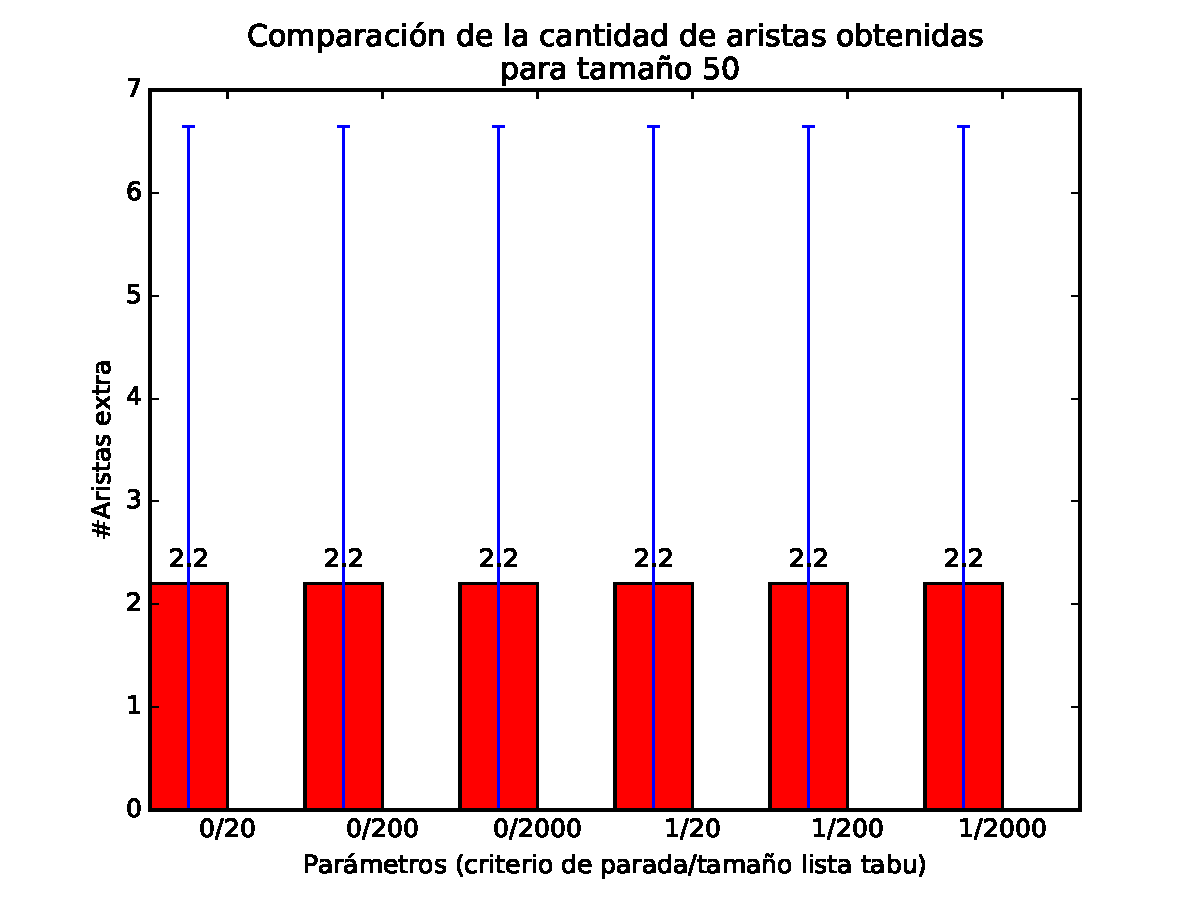
\includegraphics[width=1\textwidth]{graficos/problema_6/calidad0.pdf}
  \caption{\footnotesize{}}
  \label{fig:calidad5-1}
\end{minipage}%
\hspace{0.01\textwidth}
\begin{minipage}{0.49\textwidth}   
  \centering
    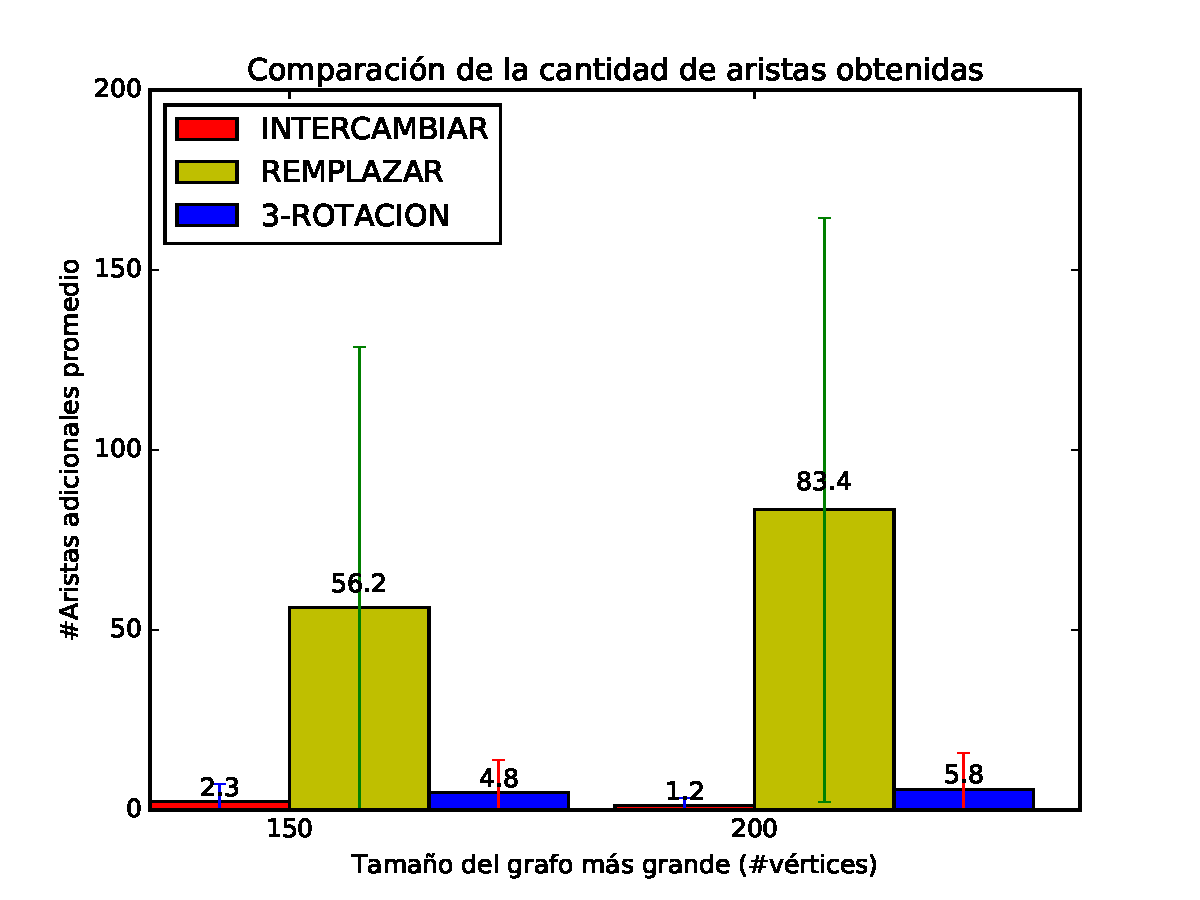
\includegraphics[width=1\textwidth]{graficos/problema_6/calidad2.pdf} 
  \caption{\footnotesize{}}
  \label{fig:calidad5-2}
\end{minipage}

\begin{minipage}{0.49\textwidth}
  \centering
    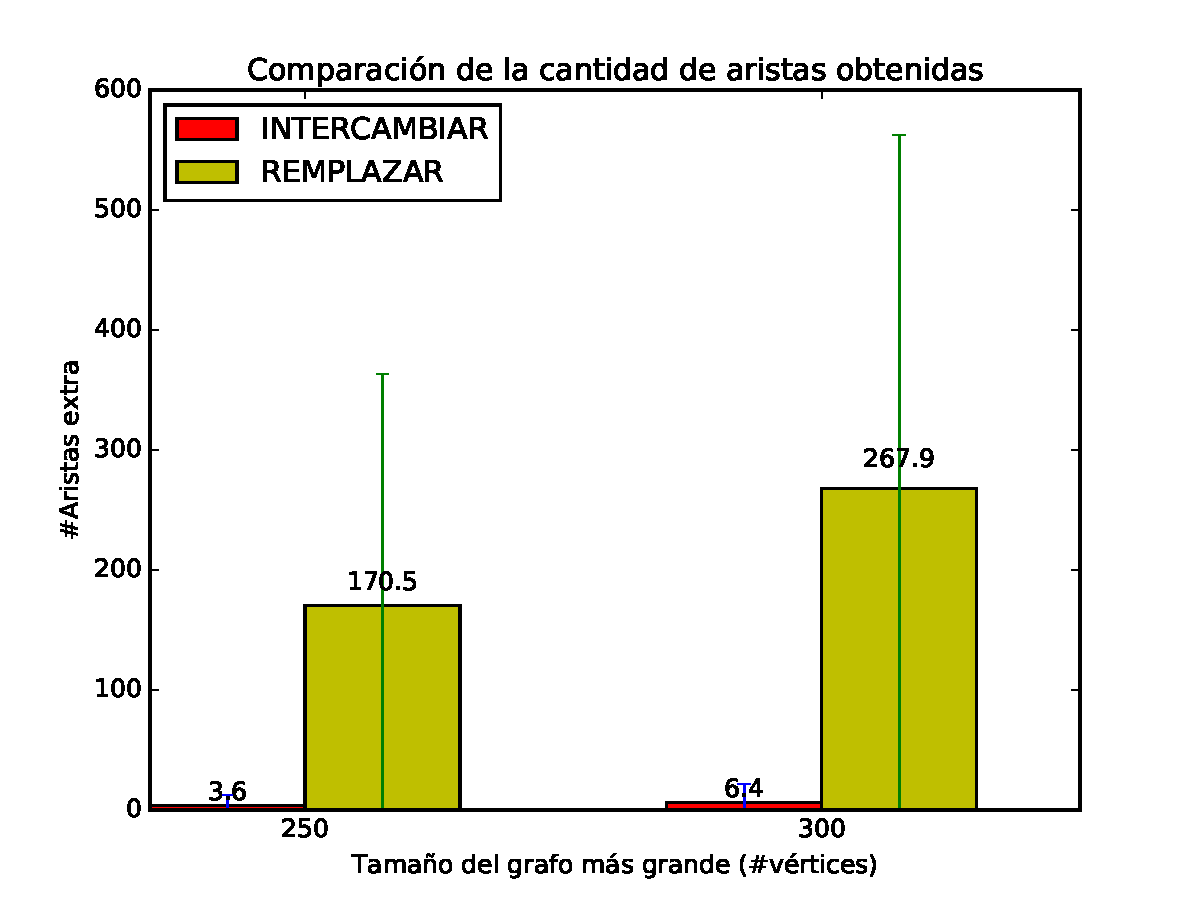
\includegraphics[width=1\textwidth]{graficos/problema_6/calidad4.pdf}
  \caption{\footnotesize{}}
  \label{fig:calidad5-3}
\end{minipage}%
\hspace{0.01\textwidth}
\begin{minipage}{0.49\textwidth}   
  \centering
    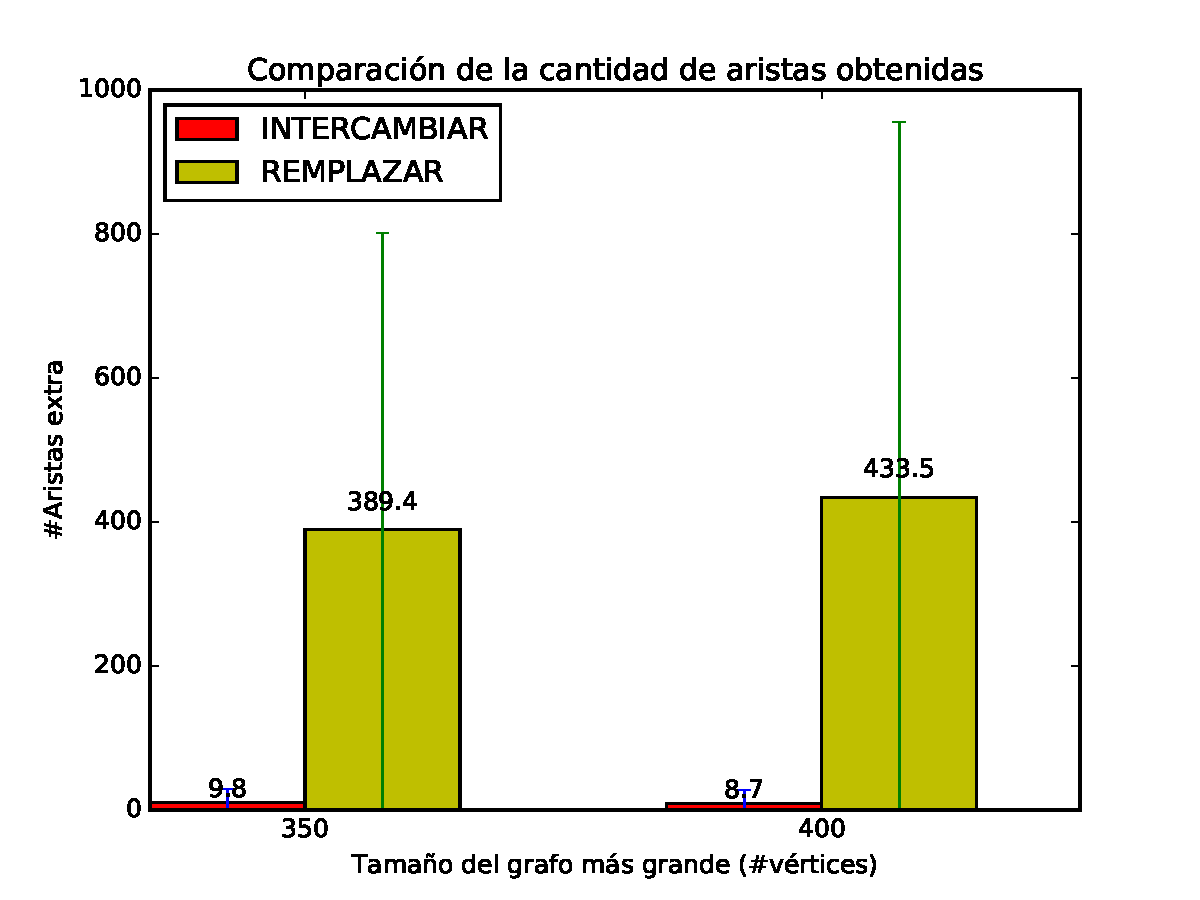
\includegraphics[width=1\textwidth]{graficos/problema_6/calidad6.pdf} 
  \caption{\footnotesize{}}
  \label{fig:calidad5-4}
\end{minipage}

\begin{minipage}{0.5\textwidth}   
  \centering
    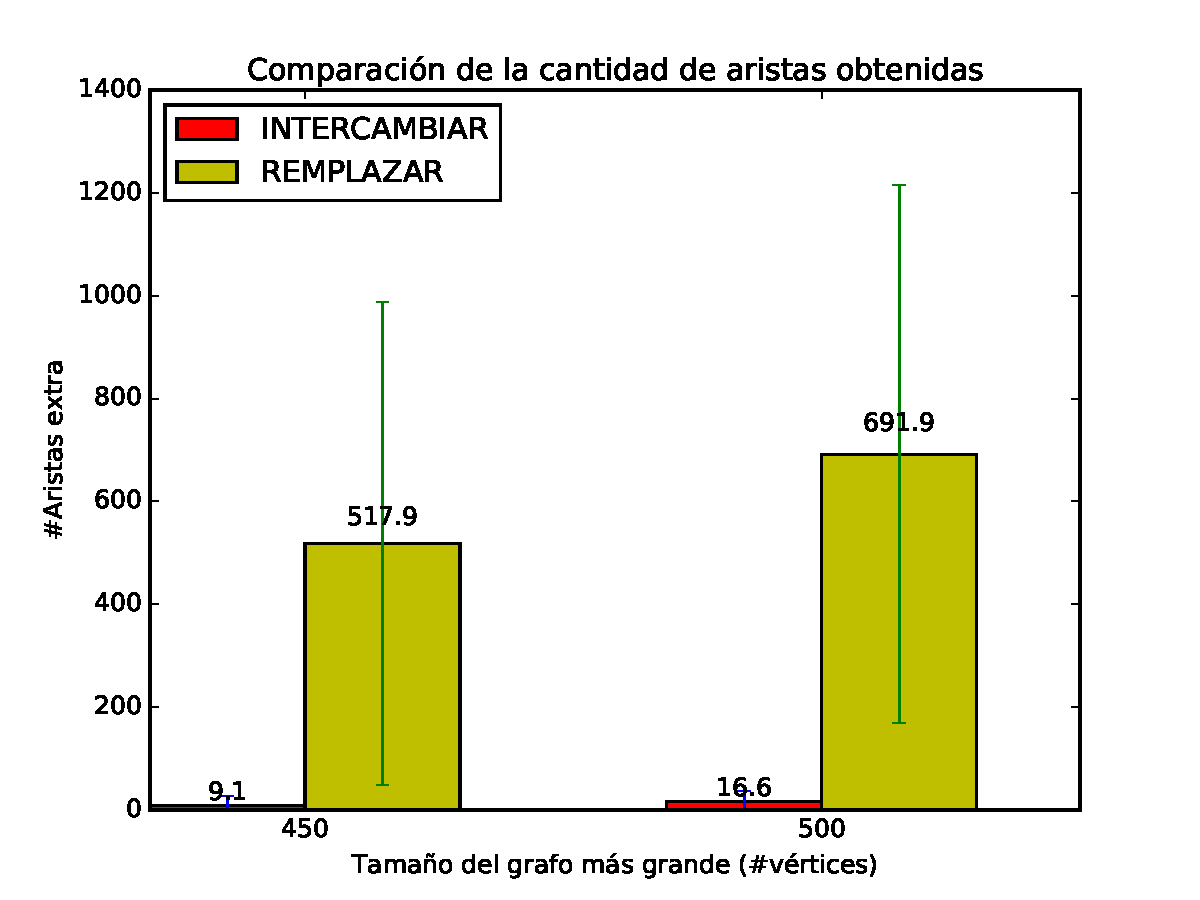
\includegraphics[width=1\textwidth]{graficos/problema_6/calidad8.pdf} 
  \caption{\footnotesize{}}
  \label{fig:calidad5-5}
\end{minipage}
\end{figure}


%%%%%Cociente%%%%%
\begin{figure}[H]
\centering
\begin{minipage}{0.49\textwidth}
  \centering
    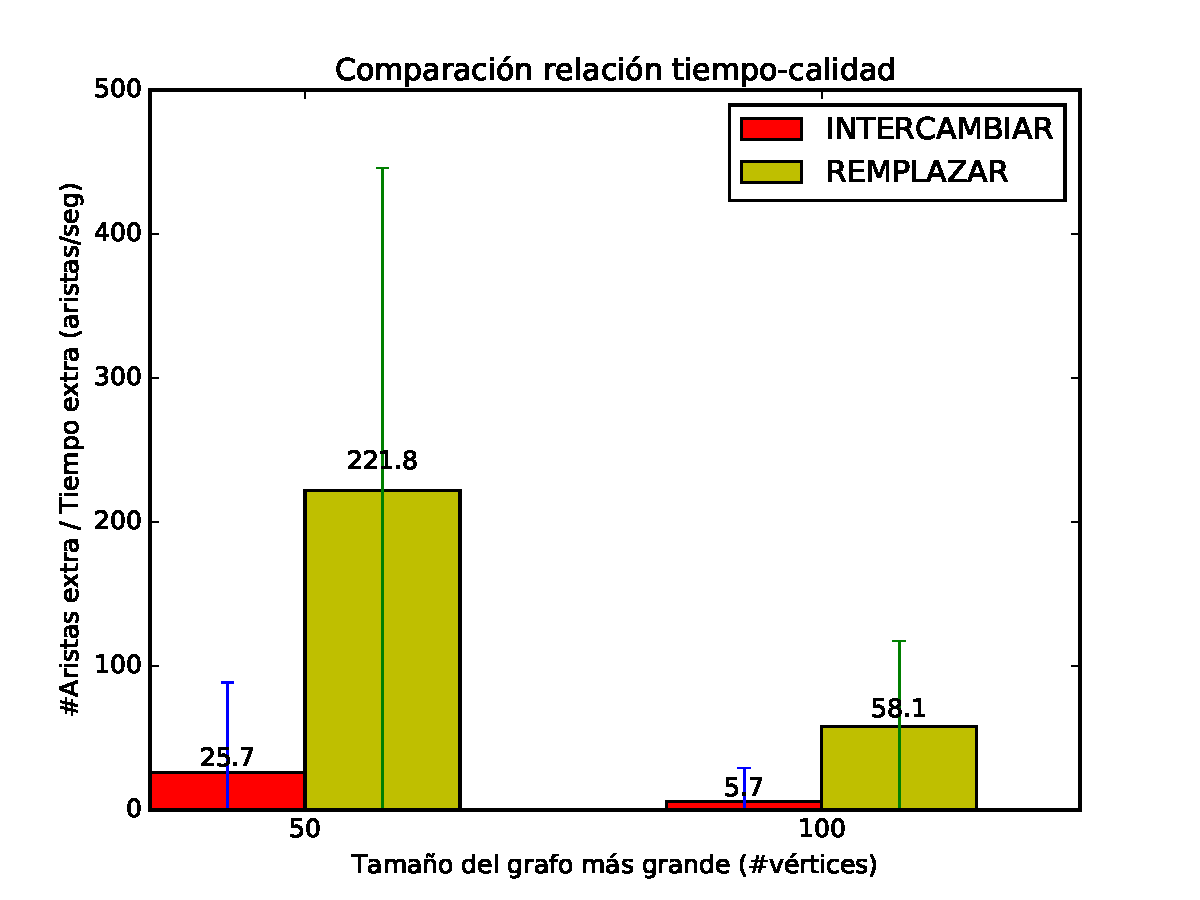
\includegraphics[width=1\textwidth]{graficos/problema_6/cociente0-0.pdf}
  \caption{\footnotesize{}}
  \label{fig:calidad5-1}
\end{minipage}%
\hspace{0.01\textwidth}
\begin{minipage}{0.49\textwidth}   
  \centering
    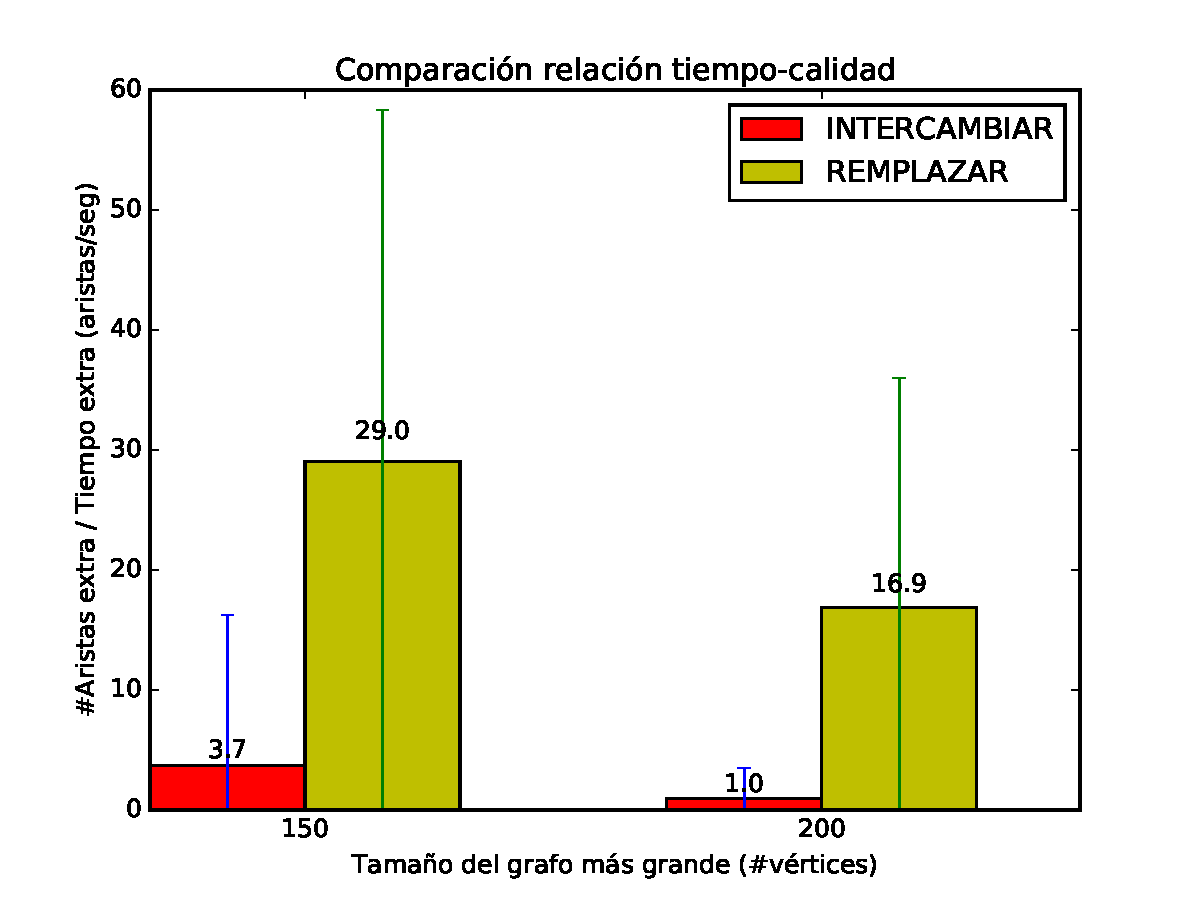
\includegraphics[width=1\textwidth]{graficos/problema_6/cociente0-2.pdf} 
  \caption{\footnotesize{}}
  \label{fig:calidad5-2}
\end{minipage}

\begin{minipage}{0.49\textwidth}
  \centering
    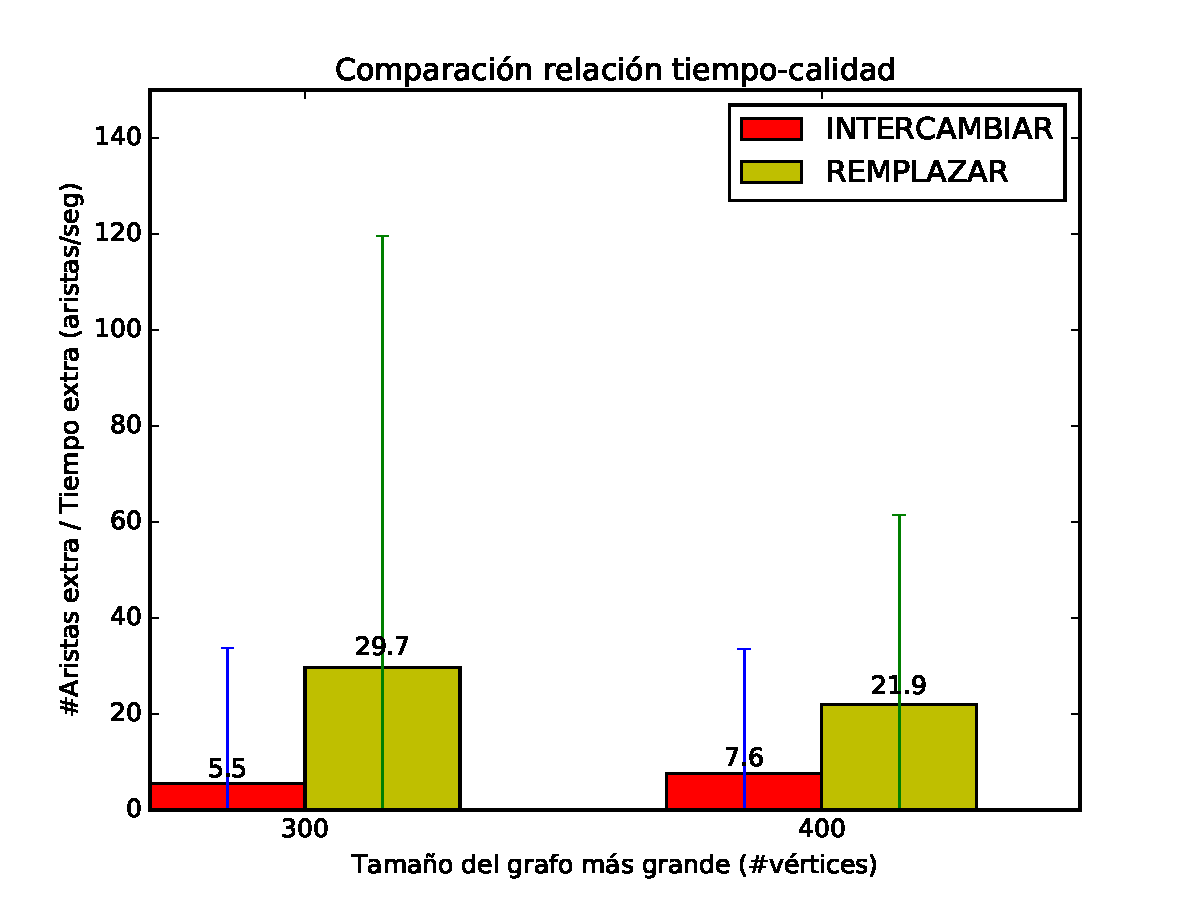
\includegraphics[width=1\textwidth]{graficos/problema_6/cociente0-4.pdf}
  \caption{\footnotesize{}}
  \label{fig:calidad5-3}
\end{minipage}%
\hspace{0.01\textwidth}
\begin{minipage}{0.49\textwidth}   
  \centering
    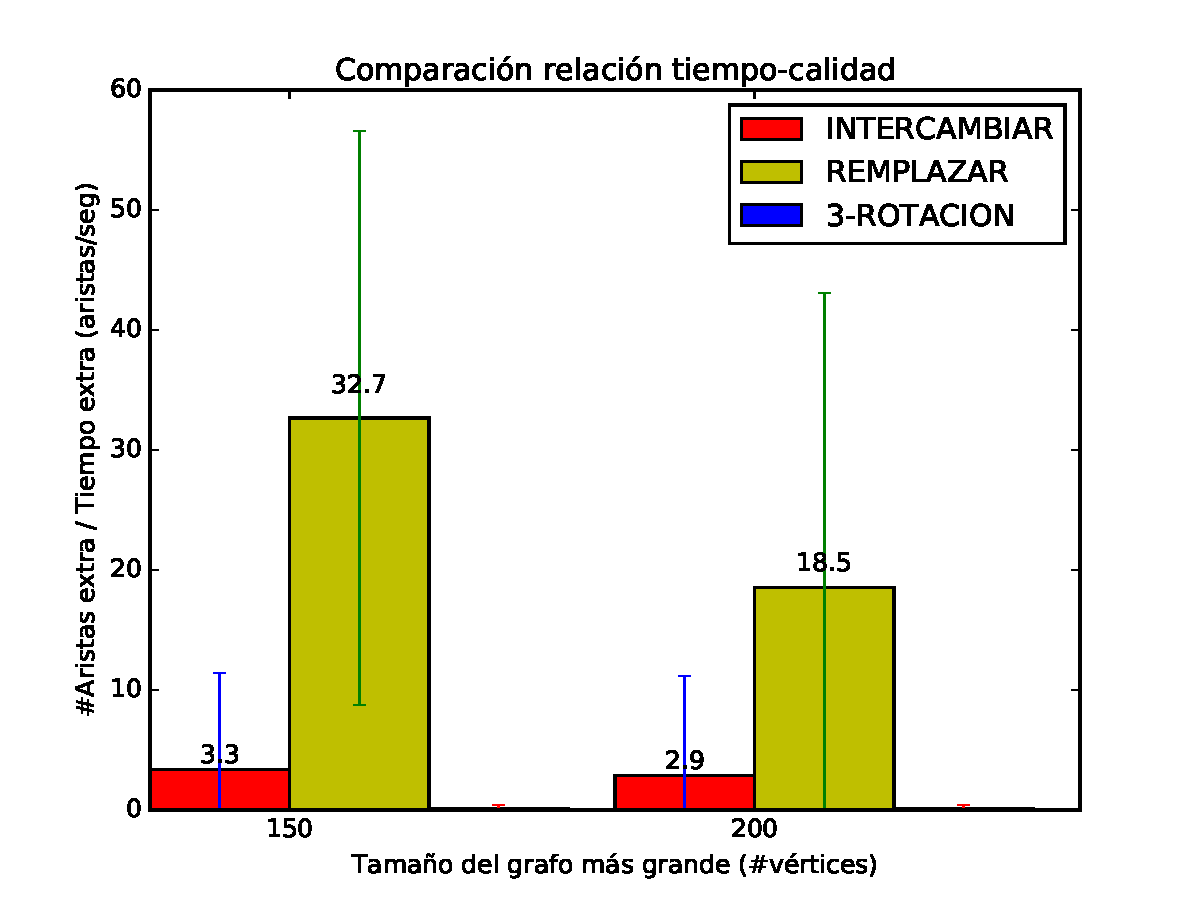
\includegraphics[width=1\textwidth]{graficos/problema_6/cociente1-2.pdf} 
  \caption{\footnotesize{}}
  \label{fig:calidad5-4}
\end{minipage}
\end{figure}


\begin{figure}[H]
  \centering
  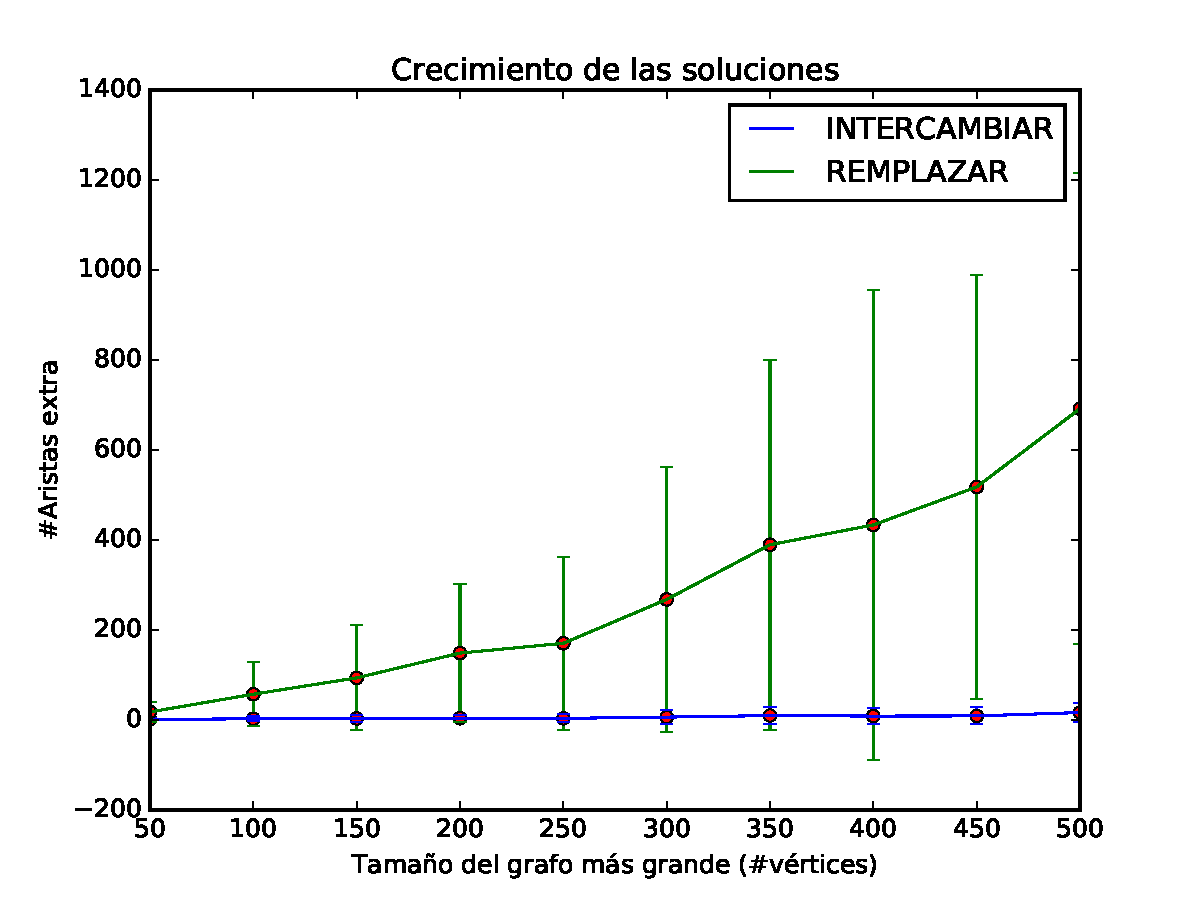
\includegraphics[width=1\textwidth]{graficos/problema_6/crecimiento.pdf} 
  \caption{\footnotesize{}}
  \label{fig:crecimiento}
\end{figure}